\documentclass{sig-alternate-05-2015}
% The following 3 lines are necessary to get rid of the automatically added and reserved space for copyright. 
\makeatletter
\def\@copyrightspace{\relax}
\makeatother
%\usepackage{float}
%\usepackage{multirow}

\graphicspath{ {./figures/} }

\begin{document}

\title{Implementing and Evaluating Stock QUIC Client/Server Performance on DPDK TCP/IP Stack}

\numberofauthors{2}
\author{
% 1st. author
\alignauthor X.D. Zhai
       \email{xingdaz@andrew.cmu.edu}
% 2nd. author
\alignauthor Spencer Baugh 
		\email{sbaugh@andrew.cmu.edu}
}

\maketitle
\begin{abstract}
\iffalse
QUIC (Quick UDP Internet Connection) is a new transport layer protocol designed and built by Google in an effort do deliver shorter latency in web loading and video watching experience for their Youtube services. Most notably, it combines crypto and transport handshakes, reducing the time for connection establishment to commonly 0-RTT. QUIC runs in user space as opposed to kernel space, allowing for fast experimentation with protocol. The protocol implementation is folded into the greater Chromium project which comes with a stock client/server to demonstrate the protocol. They are built on top of linux's network stack. In this project, we swapped out linux's network stack with one that is built on top of DPDK (called dpdk-ans) and compared the stock client/server's performance on both linux TCP stack and dpdk-ans. In addition, a similar TCP client/server is also build for comparison. We found blah blah results.
\fi
\end{abstract}

\section{Introduction}
\iffalse
QUIC is a new multiplexed and secure transport atop UDP build with HTTP/2 as the primary application protocol. I was desgined from the ground up by Google to deliver shorter latency in web loading and video watching experience for their Youtube services. It avoided all the pitfalls of TCP that make it unsuitable as a transport layer protocol in the modern web era. Put it another, QUIC = TCP + TLS + SPDY with purportedly better performance. Most notably, QUIC provides multiplexing and flow control semantics equivalent to HTTP/2 so HTTP/1 can run on QUIC yielding similar performance gain as HTTP/2, and connection can be established with fewer RTT as TCP.
\fi

\section{Background}
Our web experience is largely dominated by two factors: how fast the website loads, and how native and instantaneous the interaction feels. The former is determined by the latency of the plumbing, i.e. the network infrastracture, while the latter can be ascribed to the design, architecture and the engineering of the particular web service. To systemically and universally improve the experience, making the plumbing better is crucial. 

From the bottom up, companies like Google, Facebook and Netflix have either utilized Content Distribution Networks(CDNs), or deployed their own, to bypass the middle mile, shorten the last mile and bring the content closer to the user. From the top down, Google's Chrome web browser has employed numerous software optimizations such as speculatively querying DNS, establishing TCP connections, and even firing off resource requests based on learned user traffic patterns to minimize the latency on the browser end.\cite{grigorik:chrome} 

What is left in the middle are the stacks of protocols in need of overhaul for the modern web, and the people from Google are at it again. First, they developed the application layer protocol SPDY to address the pitfalls, particularly relating to latency, of HTTP/1.1 for delivering web pages. The motivation is that changes to transport layer are difficult to deploy because they all live in kernel space, and you get more bang for the buck if all the obvious and egregious handicaps in HTTP/1.1 can be addressed. Table~\ref{tab:httpvspdy} shows some of them and SPDY's remedy.

\vspace*{-10pt}
\begin{table}[h]
\centering
\caption{HTTP/1.1 v.s. SPDY\cite{spdy}}
\label{tab:httpvspdy}
\begin{tabular}{|r|l|}
\hline
HTTP/1 & SPDY \\ \hline
Single request per TCP connection & Multiplexed streams \\ \hline
Exclusively client-initiated requests & Server push \\ \hline
Uncompressed headers & Compression \\ \hline
Redundant headers & Elimination \\ \hline
\end{tabular}
\end{table}

On the client side, the Chrome browser has support for SPDY, and on the server side, Google donated the \texttt{mod\_spdy} to the Apache HTTPD codebase to support the protocol. Benchmark testing revealed a 64\% reduction in page loading over traditional HTTP/1.1. The SPDY protocol eventually formed the foundation of HTTP/2.

Google's quest for a faster web did not stop at the application protocol layer and the effort eventually spilled into the transport layer. If the main assumption in developing SPDY was ``well, there is nothing we can do about suboptimal networking stack, let's do our best to optimize the application protocol,'' then the implicit assumption this round is ``there is nothing we can do about the speed of light, let's reduce the number of trips needed for a connection.''\cite{quic:announcement} Having realized that developing a kernel implementation of the new protocol would be slow for experimentation and deployment, the QUIC developers decided to have this new protocol live in userland and employ UDP layer to move its packets. 

Since its stable release in April 2014, Google has ramped up the QUIC traffic to Google's services and analyzed its performance on a larger scale. Its empirical data suggest that it is 5\% faster on page load on average, mostly due to 0-RTT connection establishment, and 30\% less rebuffering for Youtube videos attributable to better handling of packet loss and stream level flow control.\cite{quic:presentation}

\begin{figure}[bh]
\centering
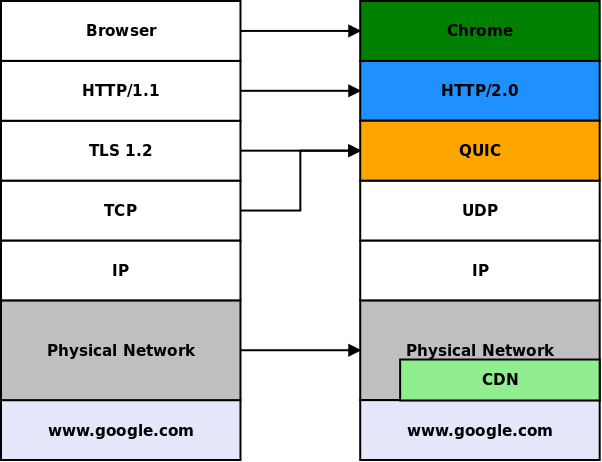
\includegraphics[scale=0.27]{web.png}
\caption{Efforts to make the web go faster}
\label{fig:webstack}
\end{figure}

Figure \ref{fig:webstack} shows a rather promising landscape. It seems that what is standing between us and the promised land of seamless web experience, at least from a networking perspective, are the speed of light (which we can't change), and how fast raw bytes on the wire are processed by the kernel and handed to the application. That is where Intel's DPDK comes in. Data Plane Development Kit, first and foremost, is not a networking stack; it does not provide the ease and comform of Layer-3 forwarding, IPsec, firewalling, etc. It is a collection of low level libraries, NIC drivers and a runtime environment living alongside the kernel for building custom applications in need of lightening fast packet processing.\cite{dpdk:home} Notably, pfSense laid out a roadmap where the core of it will be rewritten with DPDK to run at the line rate of 10Gbps interfaces. \cite{pfsense:roadmap}

Hence, it is our intention to investigate if QUIC's stock client/server performance can be further elevated using DPDK. In this project, we make 4 main contributions:

\begin{enumerate}
	\itemsep0em
	\item Compare and contrast the difference between QUIC and TCP.
	\item Explore and explain the QUIC protocol implementation and that of stock client server in the chromium source code.
	\item Explore and explain the architecture of DPDK and DPDK-ANS.
	\item Replace all Kernel UDP socket calls in the stock implementation with those of DPDK-ANS. Measure and evaluate the performance on both Linux networking stack and DPDK-ANS, against a TCP equivalent.
\end{enumerate}

\section{QUIC v.s. TCP}
As a transport layer protocol developed from the ground up, QUIC is packed with new features aimed at incorporating application layer workarounds to TCP's shortcomings(e.g. HTTP/2's stream multiplexing), fixing inherent TCP problems(e.g. retransmission ambiguity), and optimizing for low latency and security.

\subsection{Multiplexing and Flow Control}
QUIC transplanted two important features from HTTP/2 and implemented them natively in the transport layer: stream multiplexing and dedicated flow controls.

HTTP/2 multiplexes many streams on top of TCP's single byte stream abstraction, but it still suffers from head of line blocking. Within a single TCP connection, there is no distinction between packets of different streams and a lost packet from one stream is still backed up behind those from a stalled one. In QUIC, multiple streams share the same connection and some streams can always make progress in the event of lost packets in others. As a result, QUIC also implements flow control on both the stream level and the connection level. A QUIC receiver keeps track of and advertises the window size for each stream to the sender, as well as the aggregate buffer size, bytes received and offset data. \cite{quic:draft}

\subsection{Connection establishment}
Traditionally, the TCP 3 way handshake is the unavoidable cost of doing business on the web. A further 1.5 RTT is required to establish TLS. When all is said and done, 3 RTTs are wasted before application data actually flows. This is a very low hanging fruit for QUIC to pick off. 

QUIC boasts of a 0 RTT for connection establishment largely based on the assumption that the client has talked to the server before and cached the server's configuration. Otherwise, it combines crypto with handshake in a dedicated stream(Stream ID 1) to initiate a connection.

The client sends an initial inchoate hello (CHLO) to the server, specifying among other things, the common certificates it already possesses and cached certificates from previous interaction with the server(if there are any). This allows the server to not send back the whole certificate chain later. The server responds with a rejection (REJ) containing most importantly, server configuration (SCFG), in which it provides a list of available key exchange algorithms and their corresponding public values. Then the client picks an algorithm and its own corresponding public value and resends the CHLO. At this point, the client doesn't even wait for the server's reply and immediately starts sending encrypted application data. \cite{quic:crypto}

\subsection{Congestiong Control}
QUIC does not reinvent the wheel when it comes to congestion control. At the time of this writing, it uses a modified implementation of TCP Cubic which is optimized for networks with high bandwidth and high latency. Since Linux 2.6.13, TCP Cubic is the default in the standard Linux distribution. QUIC expands on the TCP Cubic and primarily offers three advantages\cite{quic:draft} over it:

\begin{enumerate}
	\itemsep0em
	\item All packets carry a new sequence number, avoiding the TCP retransmission ambiguity problem for RTT estimation.
	\item All ACKs carry delay information between the receipt of the packet and the ACK being sent. Together with the monotonically increasing packet number, precise RTT can be calculated by the other endpoint.
	\item ACKs support up to 256 NACK ranges, providing richer signaling than TCP in the event of packet reordering by the network.
\end{enumerate}

\subsection{Full Authentication and Encryption}
A well known security problem of TCP is that its headers are in plaintext and not authenticated, susecptible to injection and manipulation, by either attackers or middleboxes. Because QUIC packets ride on UDP datagrams, its packets are always authenticated and the payload is encrypted after the handshake. \cite{quic:draft}

\subsection{Connection Migration}
TCP connection is identified by the tuple \texttt{source address:port, destination address:port} specifying the end hosts, but not the logical connection between the client application and the web services it is accessing, making TCP unfriendly to mobile clients, e.g. a cell phone steps off WiFi network onto LTE or a laptop moving from one AP to another AP. QUIC addresses this problem by having the client assign a randomly generated 64-bit ID to the logical connection and it outlives all the migrations, enabling uninhibited migration across networks. \cite{quic:draft}

\section{DPDK and DPDK-ANS}
DPDK is born out of a marriage between the need for software level packet processing at line rate on commodity hardware and continued enhancements introduced by newer generations of Intel microarchitecture. The reality is that NICs at 1/10/40/100 Gb are not uncommon on servers these days but plain vanilla linux kernel is ill equipped to unleash all of their potential. On the other hand, Intel increasingly offers hardware optimizations that promises high performance packet processing but are left mostly untapped by applications. As a result, Intel embedded those features into a set of library with simple API interface and a low overhead run time environment for application developers. Table \ref{tab:dpdkchallenges} summarizes the challenges and how DPDK overcome them. \cite{dpdk:presentation}

\begin{table*}[]
\centering
\caption{Overcoming challenges of line rate packet processing in commodity hardware}
\label{tab:dpdkchallenges}
\begin{tabular}{|r|p{4in}|}
\hline
\textbf{Challenges} & \textbf{DPDK's optimizations}                                                           \\ \hline
OS can't keep up with NIC I/O interrupts & Poll Mode Drivers for NICs                                                                    \\ \hline
Context switch has high overhead & Bind a SW thread to a HW execution context, and the thread runs to completion.                               \\ \hline
\centering{Memory \& PCIe access is slow} & Perform batch read to amortize latency. Use SW or HW controlled prefetching. Align data structure to cache line size to minimize bandwidth usage. Ensure contiguous memory access in cache line size increments to minimize cache misses from evictions. Use Direct Data IO for PCIe access and read straight to cache.\\ \hline
Locks/semaphores have high overhead & Use lock free data structures. \\ \hline
Page faults are costly & Use 2MB or 1G Huge Pages in Linux to reduce TLB misses. \\ \hline
\end{tabular}
\end{table*}

DPDK's architecture can largely be broken down into 3 main components: data plane libraries and poll mode drivers(summarized in Table \ref{tab:dpdkcorelibs}), run time environment and the Environment Abstraction Layer(EAL). The run time environment is extremely low overhead and assigns core affinities to software threads which is allowed to run to completion. EAL is a service layer that provides its core libraries and applications a generic interface to system resources such as NICs, memory and PCI bus access, and logging. It straddles user space and kernel space. \cite{dpdk:programmerguide}

\vspace*{-10pt}
\begin{table}[h]
\centering
\caption{DPDK core libraries}
\label{tab:dpdkcorelibs}
\begin{tabular}{|r|p{2in}|}
\hline
Core libraries      & Description                                                                                                                                       \\ \hline
Memory Manager      & Allocate memory pools mapped to huge pages. Provides helper methods to pad data objects, stored in rings, for cache alignment and evenly distribute them on DRAM channels \\ \hline
Buffer Manager      & Pre-allocate fixed size buffers stored in pools.                                                                                                  \\ \hline
Queue Manager       & Implements lock free queues for fast access                                                                                                       \\ \hline
Flow classification & Utilizes Intel streaming SIMD intrinsics for hash based flow classification                                                                       \\ \hline
Poll Mode Drivers    & 1GbE and 10GbE NIC drivers that work without asynchronous, interrupt-based signaling mechanisms                                                   \\ \hline
\end{tabular}
\end{table}

It is clear that DPDK only offers the highly optimized building blocks of a networking stack but just not an implemented one for us to use. It so happens that there is one on the market -- DPDK Accelerated Network Stack(\texttt{dpdk-ans}). It is a port of FreeBSD's TCP/IP stack to be run in userspace as a DPDK application and it offers a subset (as it is still in active development) of the familiar set of socket API's we've come to love.

ANS fully utilizes DPDK's features. For example, it requires zero copy between NIC and the application. On NICs that support Receiver Side Scaling(RSS), the NIC distributes packets to different logical cores so that the same TCP flow go through the same core, minimizing the need for copying between cores. In addition, each core has its own UDP or TCP stack, making the implementation lock free. In addition, the socket layer tries to evenly distribute sockets to different logical cores so as to maximize the benefits of parallel processing. If there are two applications each using a socket, or a single application using two sockets, those sockets would be put on different cores. Figure \ref{fig:dpdk-archi} presents the complete picture of the logical building blocks of the DPDK TCP/IP stack. \cite{dpdkans:readme}
 
While DPDK-ANS promises great performance gain, it also creates its unique problems. First, its socket API is imcomplete; particularly \texttt{recvmsg} and \texttt{sendmsg} aren't implemented. Secondly, its sockets, and their associated file descriptors, do not live in kernel's universe and therefore, we cannot use system asynchronous I/O facilities such as \texttt{epoll} and rely on its analogue in the DPDK-ANS universe. These restrictions created many challenges to us when we were trying to preserse as many functionalities as we could while operating within the bound of the DPDK-ANS.
 
\begin{figure}[h]
\centering
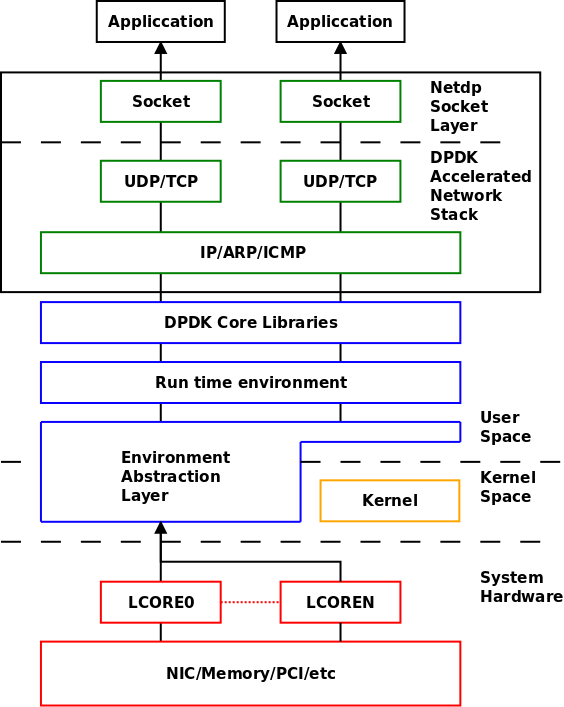
\includegraphics[scale=0.3]{dpdk_archi.png}
\caption{Overview of DPDK and DPDK-ANS architecture}
\label{fig:dpdk-archi}
\end{figure} 

\begin{figure*}
\centering
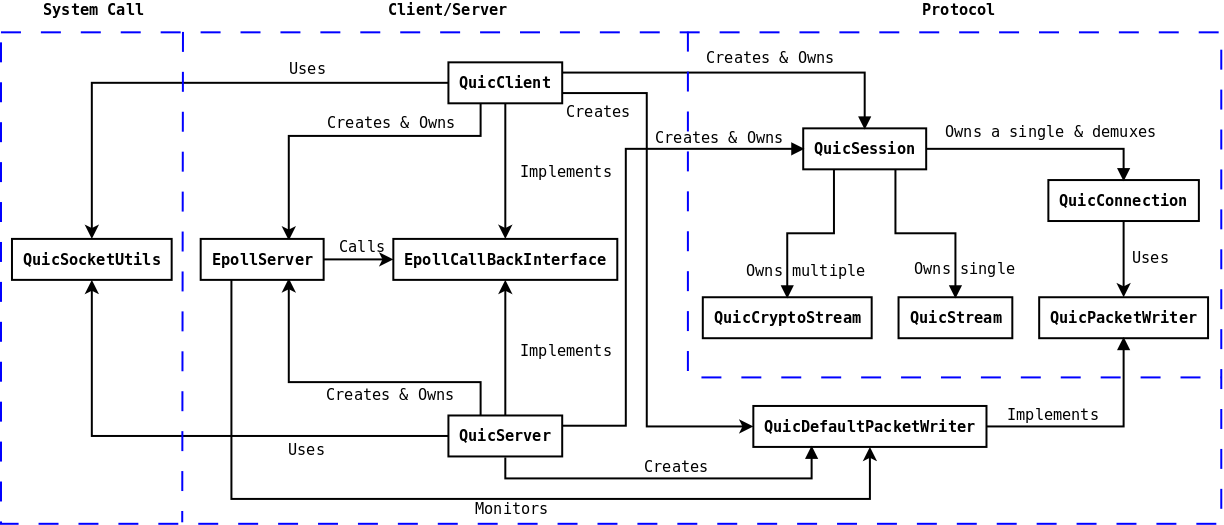
\includegraphics[scale=0.28]{class.png}
\caption{QUIC classes overview}
\end{figure*}

\section{Implementation}
The QUIC protocol is folded into the Chromium project. Shipped with it is a pair of stock client and server implementation. Our end game was to isolate the protocol from the repo and swapped out all kernel socket calls by the client/server with \texttt{dpdk-ans} ones. 
 
First, to tease out the quic protocol implementation and its dependencies into a library is no small task. Luckily, there is a third party standalone library called \texttt{libquic}\footnote{Two months after we started using \texttt{libquic}, Google released an unofficial and unsupported \texttt{protoquic} standalone library contributed by the current QUIC developers as their side project. This repo is a lot heftier than \texttt{libquic}, and sparse with documentation. We decided not to migrate over.} that is built with few modifications and patches from the Chromium project. 

Second, we have to make sure that the stock client/server still works with \texttt{libquic}. Unsurprisingly and unfortunately, we had very little success due to countless dependency issues after pulling in the stock implementations and trying to build the binary with \texttt{libquic}. Our initial progress was greatly thwarted. 

Just as we thought this project was stalled, we found out about another project called \texttt{quic\_toy} that actually used the \texttt{libquic} library for performance testing between a watered down version of the stock client/server and a simple TCP counterpart. That was our way in. 

\subsection{Source Code Overview}
Much of our time was spent on understanding the organization of the QUIC source code and looking for socket calls where the packet actually went onto the wire. Here is a overview of important classes in the implementation through the process of creating and using a \texttt{QuicClient}. \texttt{QuicServer} goes through a similiar process.

On construction, the \texttt{QuicClient} is handed a \texttt{EpollServer} and the server address. At initialization, the client creates a UDP socket, configures the socket options with utility functions from \texttt{QuicSocketUtils}, and finally registers the file descriptor and the callback \texttt{EpollCallBackInterface} functions it implements with the epoll server. Here is where most of the system calls are happening. 

After concluding with the initialization, the client attempts to connect to the server at the specified address. It first creates a                   \texttt{QuicDefaultPacketWriter} that uses, but may not own, the underlying socket file descriptor, and implements the \texttt{QuicPacketWriter} interface. Next, the client creates a \texttt{QuicConnection} and hands it a \texttt{QuicSession} that demultiplexes the connection among multiple \texttt{QuicStream}s. Lastly, the client use a dedicated \texttt{QuicCryptoStream} to perform the handshake.

If successful, the client is ready to send and receive data from the server by creating and utilizing either a single or multiple streams. Incoming packets travel from the System Call side through \texttt{epoll} callback functions to client or server and onto the underlying protocol suite where states are kept for different streams. The reverse applies for outgoing packets.

\subsection{Socket Call Replacements}
The protocol classes do not create or own any file descriptors and therefore, we are not too interested in them. On the other hand, socket and epoll system calls largely concentrated in \texttt{QuicSocketUtils} and \texttt{EpollServer}. 

%https://github.com/maufl/quic_toy
%https://github.com/devsisters/libquic
%https://github.com/google/proto-quic

\section{Benchmark Setup and Measurements}
This section presents the VM setup, tests scenarios and layout the measurement result.

\section{Evaluation}
Why did we observe what we observed?

\section{Future Work}
What we wished we did?

\section{Conclusions}

\section{Acknowledgments}


\bibliographystyle{abbrv}
\bibliography{sigproc}
\end{document}
